\documentclass[11pt]{article}

\usepackage{hyperref}
\usepackage[pdftex]{graphicx}
\usepackage{subcaption}
\usepackage{amsmath,amsfonts,amssymb}
\usepackage{hyperref}
\usepackage{rotating}
\usepackage{float}
\usepackage{color}

\setlength{\textwidth}{6.2in}
\setlength{\oddsidemargin}{0.3in}
\setlength{\evensidemargin}{0in}
\setlength{\textheight}{8.7in}
\setlength{\voffset}{-.7in}
\setlength{\headsep}{26pt}
\setlength{\parindent}{0pt}
\setlength{\parskip}{5pt}

\newcommand{\dd}{\mathrm{d}}

\title{Simple mechanism for HOC}
\author{David A. Leen, Eric Shea-Brown}
\begin{document}
\maketitle
%%%%%%%%%%%
\section{Motivation} %
%%%%%%%%%%%
\begin{enumerate}
\item DG model
\item EIF more realistic
\item Easy way of realizing higher-order correlations
\item Use of Ising model in literature
\end{enumerate}

Use of Ising model on electrophysiological data can give poor results. See Yu et al, especially for quantities like population activity, avalanches etc.

Recent work by Macke et.~al~\cite{Macke:2011gw} shows that common input gives rise to higher-order correlations in the Dichotomized Gaussian neuron model. Motivated by this finding we investigate whether the same holds true when one considers biologically plausible neuron models such as integrate-and-fire neurons.

~\cite{Barreiro:2010ud}

\begin{enumerate}
\item Ising model used on electro recordings -- results aren't great. Therefore need new statistical model... the DG model works very well [refs] but it is not clearly related to biophysics.
\item EIF model can capture higher order correlations AND the tractable reduction, does too.
\item Suggests linear point process models for higher order correlations.
\item Beyond data analysis, open problem: mechanisms which produce higher order correlations?
\end{enumerate}


%%%%%%%%%
\section{Model} %
%%%%%%%%%
\begin{enumerate}
\item Figure schematic
\item 
\end{enumerate}

The model consists of $N$ homogeneous exponential integrate-and-fire neurons receiving common white noise inputs $\xi(t)$ and independent white noise inputs $\xi_i(t)$ whose membrane voltage evolves according to the equation: 
\begin{equation}
\tau_m \frac{\dd V_i}{\dd t} = -V_i +\psi(V_i)+ \gamma+  \sigma \sqrt{\tau} \left( \sqrt{\lambda}~\xi(t) + \sqrt{1-\lambda}~\xi_i(t) \right),\quad i=1,\ldots,N.
\end{equation}
\begin{equation}
\psi(V_i) = 
\begin{cases}
0 & \text{for LIF,}  \\
\Delta_T \exp{\left(\frac{ V_i - V_S}{\Delta_T}\right)} & \text{for EIF}.
\end{cases}
\end{equation}
Here, $\tau_m$ is the membrane time constant, $\Delta_T$ controls the slope of the action potential initiation. We use the usual convention of declaring a spike whenever the voltage reaches a certain threshold $V_T$, which we have set at $-50$mV for LIF and $20$mV for the EIF neurons. The EIF neuron has an additional ``soft'' threshold, $V_S$ beyond which the voltage diverges to infinity. We set this value as $-53$mV. After a spike the voltage is reset to $V_R$, set at $-60$mV for both models, and is held there for the duration of the refractory period $\tau_{\text{ref}}$. The spikes are binned into bins of with $T_\text{bin}$, which we choose to be $10$ms.

The input current has a constant (DC) component $\gamma$, considered the effective rest potential in the absence of noise, and a stochastic component with amplitude $\sigma$. The input is modeled by a correlated Gaussian with mean $\gamma$, and covariance $\lambda$. The output spike trains have a mean $\mu$ and covariance $\alpha$. For compatibility $\mu$ describes the mean number of spikes in each bin. Following~\cite{Macke:2011gw} we define the pairwise correlation coefficient $\rho = \alpha/\text{std}^2$ [FIX].

\newpage
%%%%%%%%%%%
\section{EIF results} %
%%%%%%%%%%%
\begin{enumerate}
\item Normal axis figures as insets?
\item Plot on top of one another but mane have each different value of correlation on new plot.
\item Changing EIF parameter values only constrains $\mu, \rho$ space.
\end{enumerate}
\subsection{Using default EIF values}

%%%%%%%
% mu = 0.1  %
%%%%%%%
\begin{figure}[H]
	\begin{subfigure}[h]{0.5\textwidth}
	\centering
	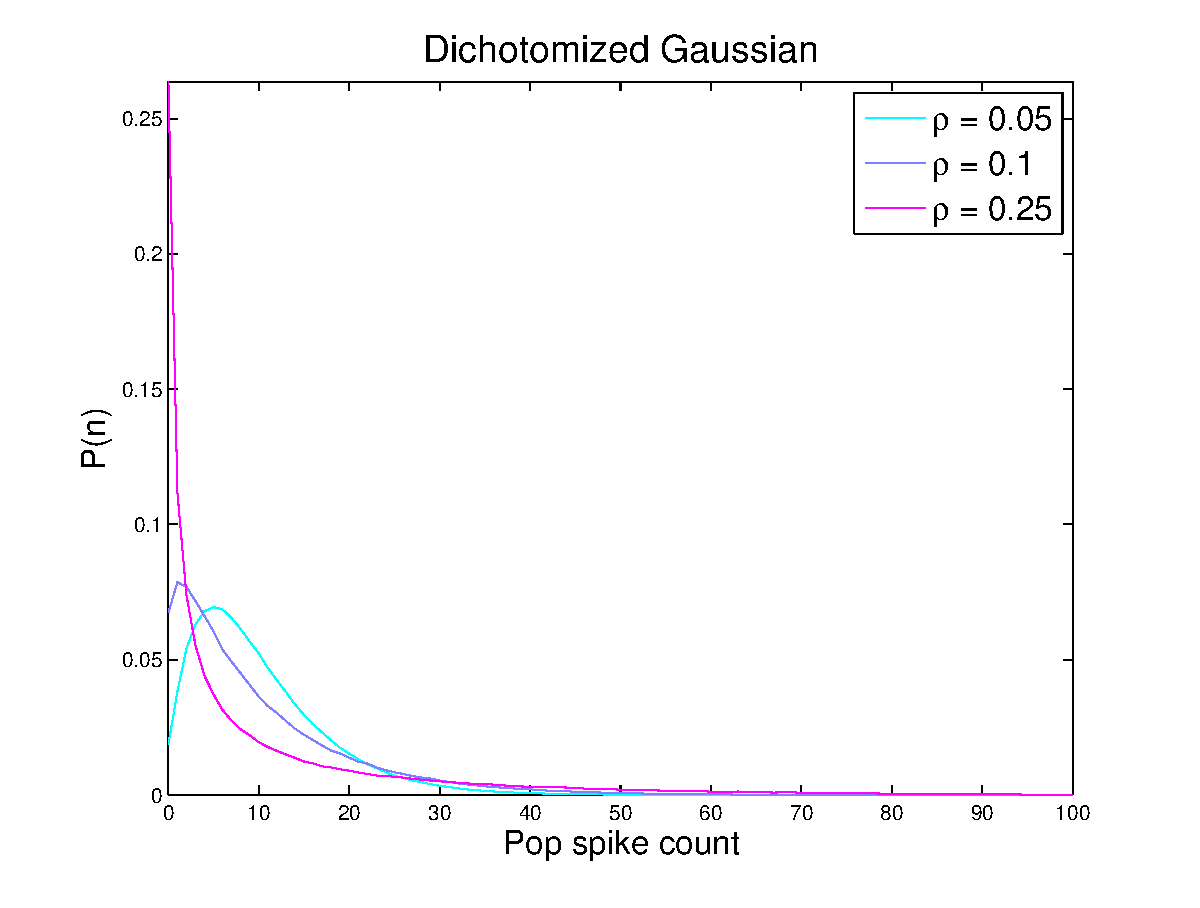
\includegraphics[width=\textwidth]{../Figures/DG/DG_Macke_2a}
	\caption{\footnotesize DG, $\mu = 0.1$, $10$ms bin.}
	\label{fig1}
	\end{subfigure}
	\begin{subfigure}[h]{0.5\textwidth}
	\centering
	\includegraphics[width=\textwidth]{../Figures/EIF/EIF_Macke_2a}
	\caption{\footnotesize EIF, $\mu = 0.1$, $10$ms bin.}
	\label{fig2}
	\end{subfigure}
	\begin{subfigure}[h]{0.5\textwidth}
	\centering
	\includegraphics[width=\textwidth]{../Figures/DG/DG_Macke_2a_semilog}
	\caption{\footnotesize DG, $\mu = 0.1$, $10$ms bin, loglinear plot.}
	\label{fig3}
	\end{subfigure}
	\begin{subfigure}[h]{0.5\textwidth}
	\centering
	\includegraphics[width=\textwidth]{../Figures/EIF/EIF_Macke_2a_semilog}
	\caption{\footnotesize EIF, $\mu = 0.1$, $10$ms bin, loglinear plot.}
	\label{fig4}
	\end{subfigure}
	\caption{\footnotesize Comparing DG with EIF using normal scale plots. Values for EIF neurons used are: bin size $10$ms, membrane time constant $\tau_m = 5$ms, refractory period $\tau_\text{ref} = 3$ms. The parameters are $\gamma = -60$mV, $\lambda = 0.17,~0.305,~\text{and}~0.514$ to give mean firing rate $\mu = 0.1$ spikes per bin and pairwise correlations $\rho = 0.05,~0.1,~\text{and}~0.25$ respectively. Values for the DG are: $\sigma = 1$, $\gamma = -1.28$, $\lambda = 0.132,~0.242,~\text{and}~0.502$.}
\end{figure}

%%%%%%%
% mu = 0.1  %
%%%%%%%
\begin{figure}[H]
	\begin{subfigure}[h]{0.5\textwidth}
	\centering
	\includegraphics[width=\textwidth]{../Figures/EIF/EIF_Macke_2a_100ms}
	\caption{\footnotesize EIF, $\mu = 0.1$, $100$ms bin.}
	\label{fig5}
	\end{subfigure}
	\begin{subfigure}[h]{0.5\textwidth}
	\centering
	\includegraphics[width=\textwidth]{../Figures/EIF/EIF_Macke_2a_100ms_semilog}
	\caption{\footnotesize EIF, $\mu = 0.1$, $100$ms bin, log-linear plot.}
	\label{fig6}
	\end{subfigure}
	\begin{subfigure}[h]{0.5\textwidth}
	\centering
	\includegraphics[width=\textwidth]{../Figures/EIF/EIF_Macke_2a_100ms_gamma}
	\caption{\footnotesize EIF, $\mu = 0.1$, $100$ms bin, $\sigma$ unchanged, $\gamma$ changed.}
	\label{fig3}
	\end{subfigure}
	\begin{subfigure}[h]{0.5\textwidth}
	\centering
	\includegraphics[width=\textwidth]{../Figures/EIF/EIF_Macke_2a_100ms_gamma_semilog}
	\caption{\footnotesize EIF, $\mu = 0.1$, $100$ms bin, $\sigma$ unchanged, $\gamma$ changed, log-linear plot.}
	\label{fig4}
	\end{subfigure}
	\caption{\footnotesize We now use a $100$ms time bin. We set $\gamma = -60$mV and change $\sigma$ to achieve a mean firing rate of $\mu = 0.1$. The value we use is $\sigma = 3.828$ compared to the original value of $\sigma = 6.23$. We have to change $\lambda = 0.29,~0.447,~0.687$ to achieve pairwise correlations $\rho = 0.05,~0.1,~\text{and}~0.25$ respectively. We notice that this is in line with previous results that increasing the bin size requires an increase in input correlation parameter. \textcolor{red}{[REF]}.\\
	In this figure to achieve a mean firing rate of $\mu = 0.1$ we kept $\sigma$ fixed at its $10$ms counterpart value of $\sigma = 6.23$mV and instead adjusted $\gamma$. To lower the firing rate in the larger bins we dropped $\gamma = -60$mV down to $\gamma = -63.8$mV. The input correlation did not need to be adjusted. There was no difference whether we tuned the mean firing rate using $\gamma$ or $\sigma$.}
\end{figure}

%%%%%%%
% mu = 0.1  %
%%%%%%%
\begin{figure}[H]
	\centering
	\includegraphics[width=0.75\textwidth]{../Figures/EIF/DG_EIF_Macke_2a_100ms_semilog}
	\caption{\footnotesize We plot the DG probability distribution over the EIF probability distribution. We fixed $\gamma$ at a value of $-60$mV, and changed $\sigma$ to achieve a mean firing rate of $\mu = 0.1$ spikes per bin. The other values are above. Alternatively, we could have kept $\sigma$ fixed and changed $\gamma$ to achieve $\mu = 0.1$. We do this in the next figure.}
	\label{figdgeif}
\end{figure}

\newpage
%%%%%%%%%%%%%%%%%%%
%%%%%%%%%%%%%%%%%%%

%%%%%%%
% mu = 0.2  %
%%%%%%%
\begin{figure}[H]
	\begin{subfigure}[h]{0.5\textwidth}
	\centering
	\includegraphics[width=\textwidth]{../Figures/DG/DG_Macke_2a_mu_02}
	\caption{DG}
	\label{fig5}
	\end{subfigure}
	\begin{subfigure}[h]{0.5\textwidth}
	\centering
	\includegraphics[width=\textwidth]{../Figures/EIF/EIF_Macke_2a_mu_02}
	\caption{EIF}
	\label{fig6}
	\end{subfigure}
	\begin{subfigure}[h]{0.5\textwidth}
	\centering
	\includegraphics[width=\textwidth]{../Figures/DG/DG_Macke_2a_mu_02_semilog}
	\caption{DG}
	\label{fig7}
	\end{subfigure}
	\begin{subfigure}[h]{0.5\textwidth}
	\centering
	\includegraphics[width=\textwidth]{../Figures/EIF/EIF_Macke_2a_mu_02_semilog}
	\caption{EIF}
	\label{fig8}
	\end{subfigure}
	\caption{\footnotesize Comparing DG with EIF using normal scale plots. Values for EIF neurons used are: bin size $10$ms, membrane time constant $\tau_m = 5$ms, refractory period $\tau_\text{ref} = 3$ms. The parameters are $\gamma = -58.2$mV, $\lambda = 0.135,~0.256,~\text{and}~0.55$ to give mean firing rate $\mu = 0.2$ spikes per bin and pairwise correlations $\rho = 0.05,~0.1,~\text{and}~0.25$ respectively. Values for the DG are: $\sigma = 1$, $\gamma = -0.84$, $\lambda = 0.1,~0.19,~\text{and}~0.435$.}
\end{figure}

\newpage
%%%%%%%%%%%%%%%%%%%%%%%
%%%%%%%%%%%%%%%%%%%%%%%

%%%%%%%
% mu = 0.3  %
%%%%%%%
\begin{figure}[H]
	\begin{subfigure}[h]{0.5\textwidth}
	\centering
	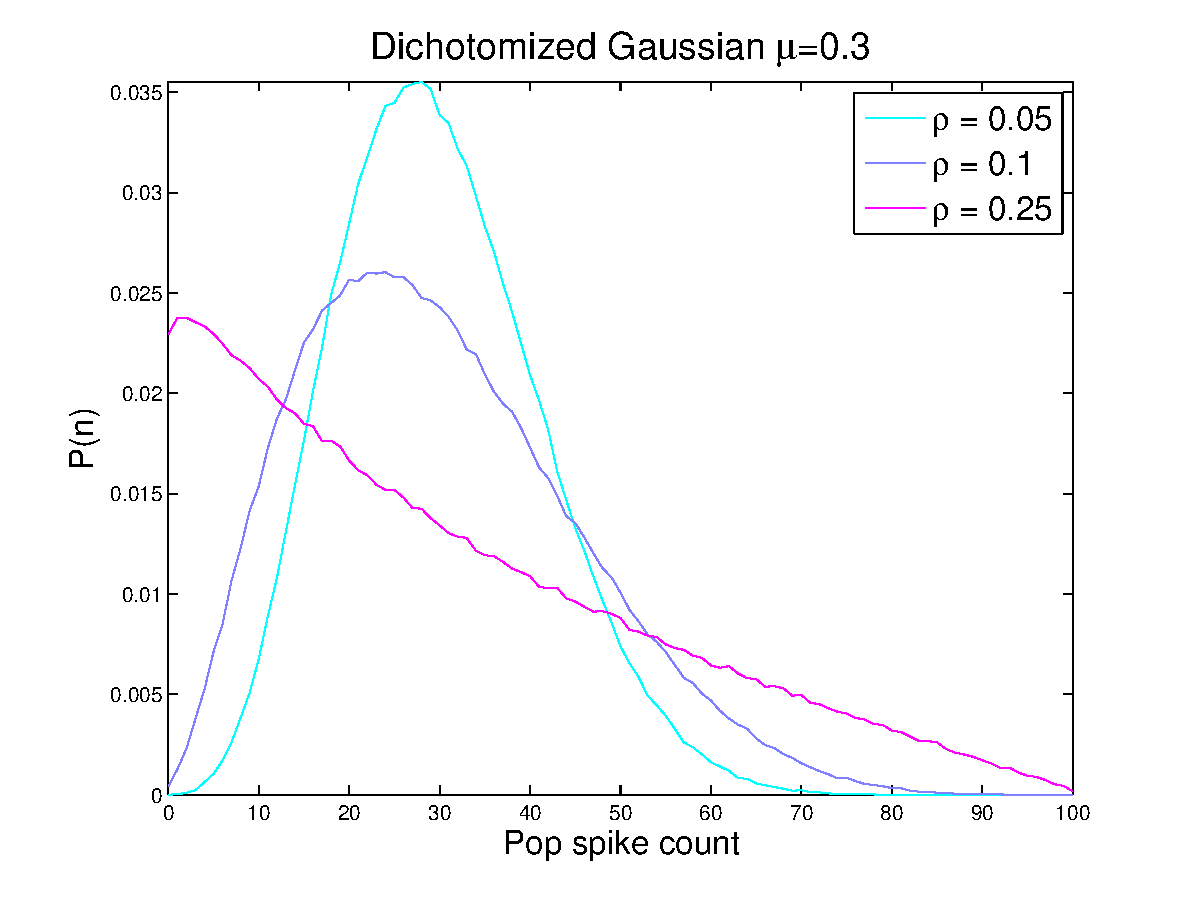
\includegraphics[width=\textwidth]{../Figures/DG/DG_Macke_2a_mu_03}
	\caption{DG}
	\label{fig9}
	\end{subfigure}
	\begin{subfigure}[h]{0.5\textwidth}
	\centering
	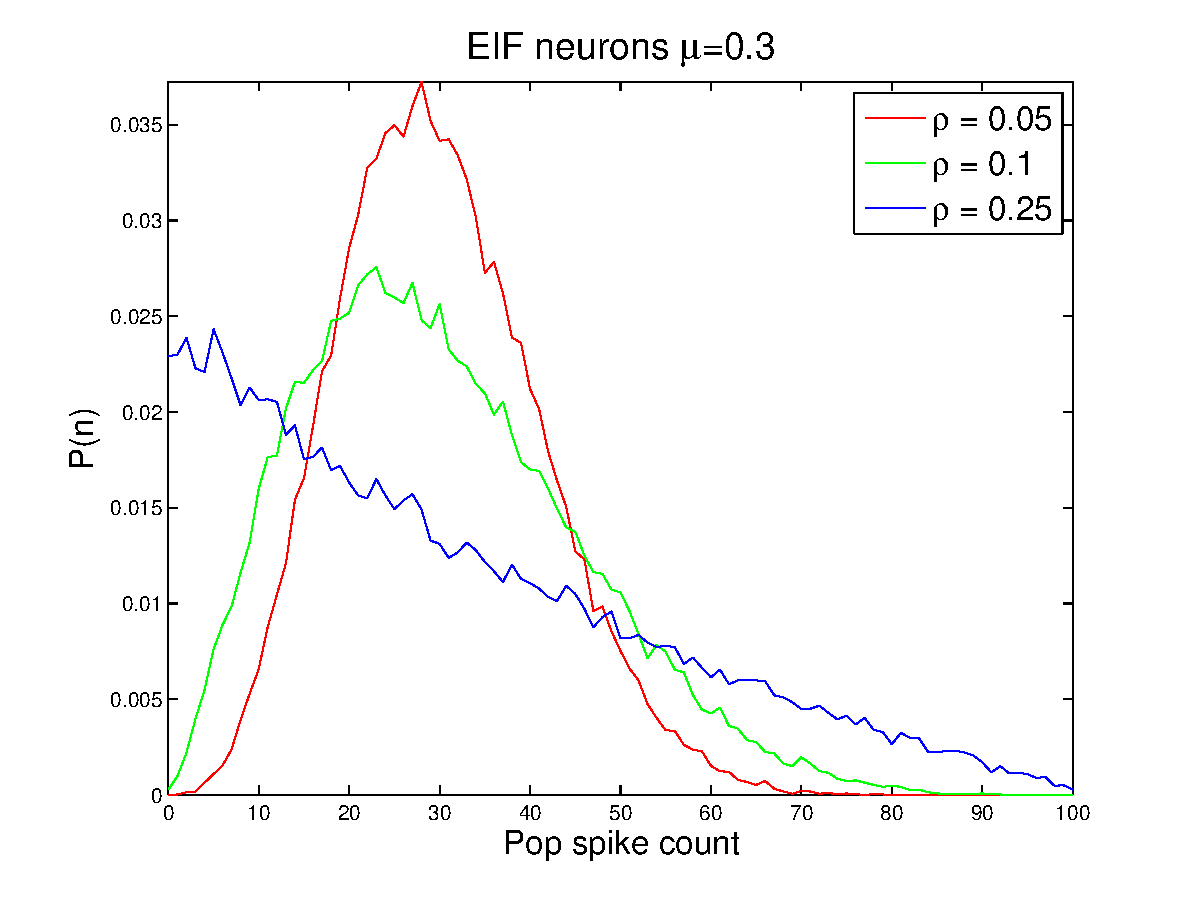
\includegraphics[width=\textwidth]{../Figures/EIF/EIF_Macke_2a_mu_03}
	\caption{EIF}
	\label{fig10}
	\end{subfigure} \\
	\begin{subfigure}[h]{0.5\textwidth}
	\centering
	\includegraphics[width=\textwidth]{../Figures/DG/DG_Macke_2a_mu_03_semilog}
	\caption{DG, semilog}
	\label{fig11}
	\end{subfigure}
	\begin{subfigure}[h]{0.5\textwidth}
	\centering
	\includegraphics[width=\textwidth]{../Figures/EIF/EIF_Macke_2a_mu_03_semilog}
	\caption{EIF, semilog}
	\label{fig12}
	\end{subfigure}
	\caption{\footnotesize Comparing DG with EIF using normal scale plots. Values for EIF neurons used are: bin size $10$ms, membrane time constant $\tau_m = 5$ms, refractory period $\tau_\text{ref} = 3$ms. The parameters are $\gamma = -56.8$mV, $\lambda = 0.12,~0.235,~\text{and}~0.529$ to give mean firing rate $\mu = 0.3$ spikes per bin and pairwise correlations $\rho = 0.05,~0.1,~\text{and}~0.25$ respectively. Values for the DG are: $\sigma = 1$, $\gamma = -1.28$, $\lambda = 0.132,~0.242,~\text{and}~0.502$.}
\end{figure}

%%%%%%%
% mu = 0.3  %
%%%%%%%
\begin{figure}[H]
\centering
\includegraphics[width=0.75\textwidth]{../Figures/EIF/DG_EIF_Macke_2a_mu_03_100ms_semilog}
\caption{\footnotesize We plot the DG probability distribution over the EIF probability distribution. We use a $100$ms time bin. Mean firing rate $\mu = 0.3$. Noise variance $\sigma = 6.23$. We set $\gamma = -62.02$mV, we use $\lambda = 0.194,~0.33,~0.609$. Is there a discrepancy here for $\rho = 0.25$? Run a much longer simulation on the server to check. }
\label{figdgeif1}
\end{figure}

\newpage
%%%%%%%%%%%%%%%%%%%%%
%%%%%%%%%%%%%%%%%%%%%

%%%%%%%
% mu = 0.5  %
%%%%%%%
\begin{figure}[H]
	\begin{subfigure}[h]{0.5\textwidth}
	\centering
	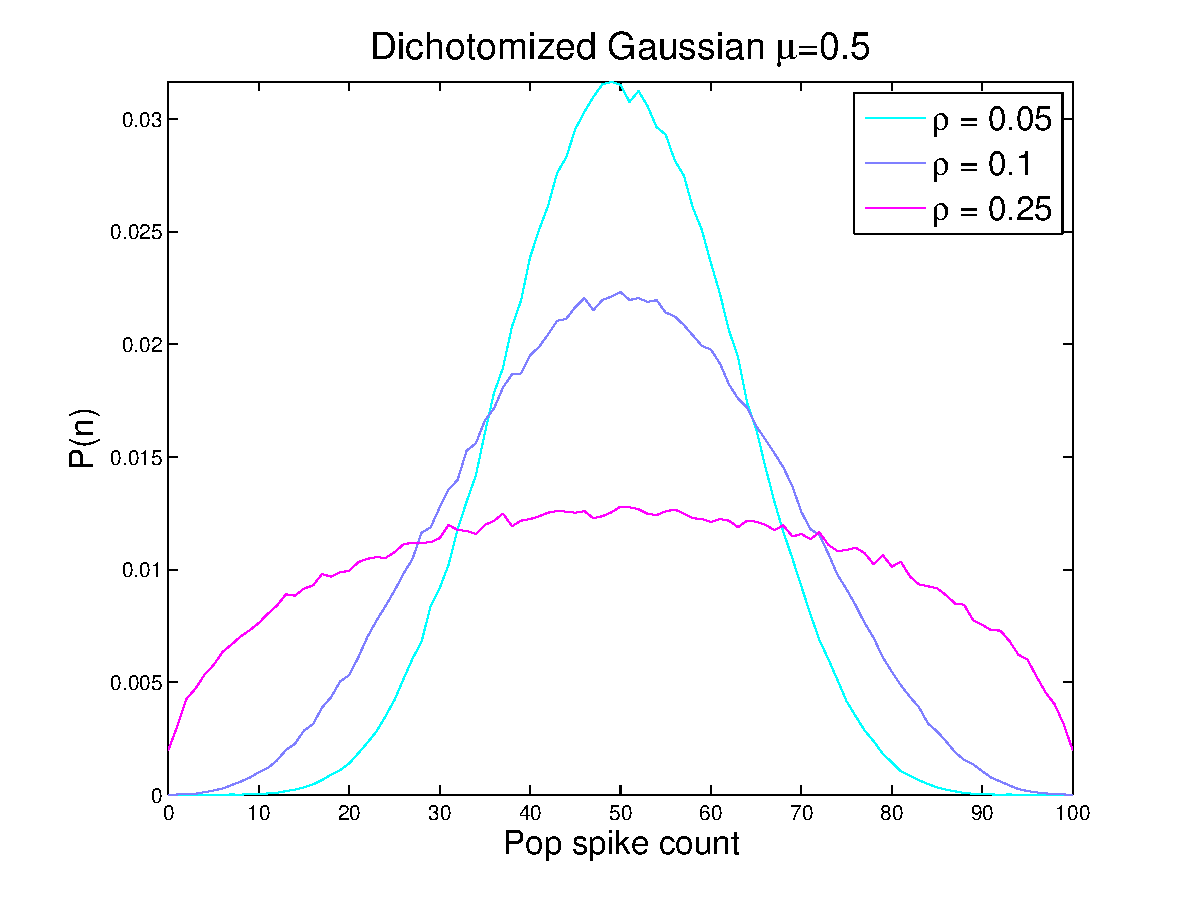
\includegraphics[width=\textwidth]{../Figures/DG/DG_Macke_2a_mu_05}
	\caption{DG, $\mu = 0.5$, $10$ms bin.}
	\label{fig11}
	\end{subfigure}
	\begin{subfigure}[h]{0.5\textwidth}
	\centering
	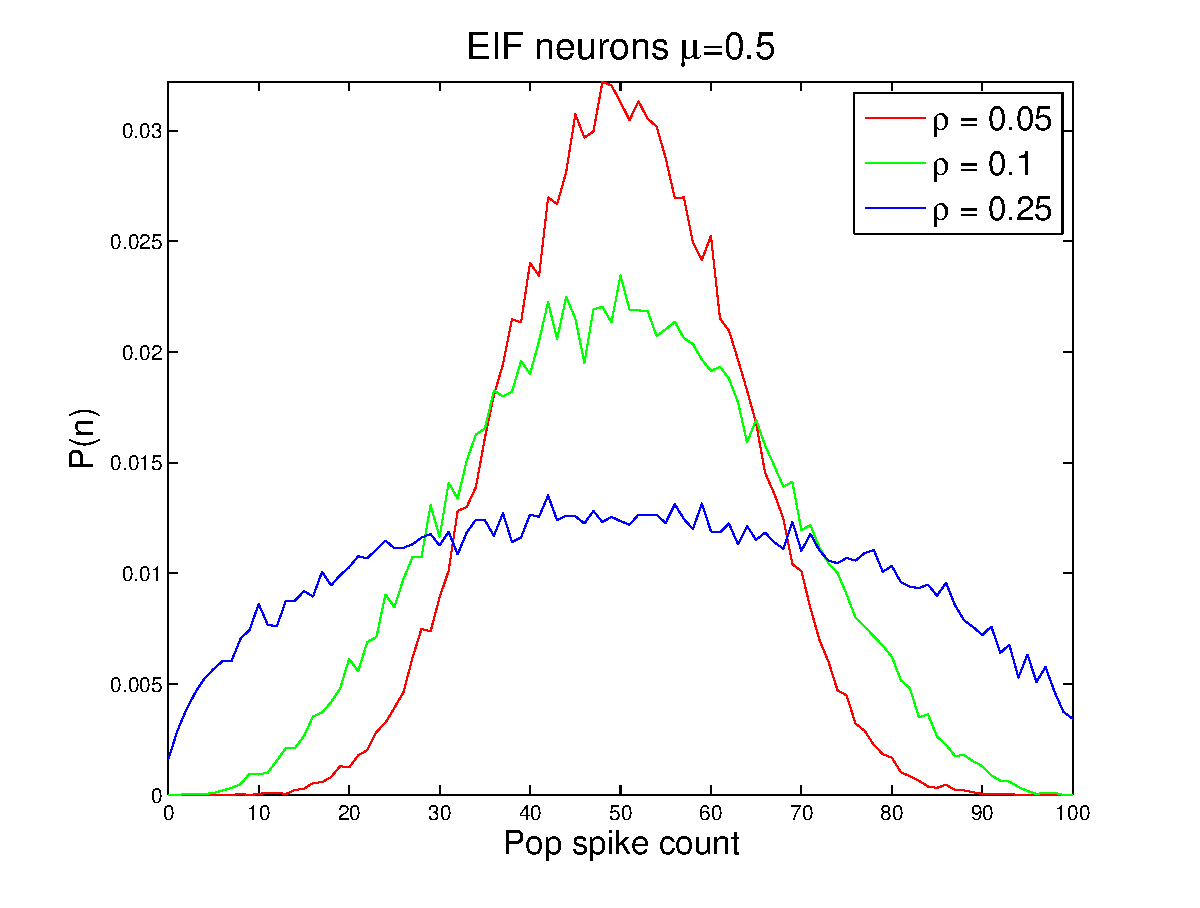
\includegraphics[width=\textwidth]{../Figures/EIF/EIF_Macke_2a_mu_05}
	\caption{EIF, $\mu = 0.5$, $10$ms bin.}
	\label{fig12}
	\end{subfigure}
	\begin{subfigure}[h]{0.5\textwidth}
	\centering
	\includegraphics[width=\textwidth]{../Figures/DG/DG_Macke_2a_mu_05_semilog}
	\caption{DG, $\mu = 0.5$, $10$ms bin.}
	\label{fig11}
	\end{subfigure}
	\begin{subfigure}[h]{0.5\textwidth}
	\centering
	\includegraphics[width=\textwidth]{../Figures/EIF/EIF_Macke_2a_mu_05_semilog}
	\caption{EIF, $\mu = 0.5$, $10$ms bin.}
	\label{fig12}
	\end{subfigure}
	\caption{\footnotesize Using normal plots. Values used in the EIF neurons: $\sigma = 6.23$, $\gamma = -54.165$mV, $\lambda = 0.118,~0.23,~0.529$. For the DG we set $\gamma = 0$ and $\sigma = 1$ as expected. We used $\lambda = 0.078,~0.157,~0.382$.}
\end{figure}

%%%%%%%
% mu = 0.5  %
%%%%%%%
\begin{figure}[H]
\centering
\includegraphics[width=0.75\textwidth]{../Figures/EIF/DG_EIF_Macke_2a_mu_05_semilog}
\caption{\footnotesize We plot the DG probability distribution over the EIF probability distribution. We use a $10$ms time bin. Mean firing rate $\mu = 0.5$. Noise variance $\sigma = 6.23$. We set $\gamma = -54.165$mV, we use $\lambda = 0.118,~0.23,~0.529$.}
\label{figdgeif}
\end{figure}

\newpage
%%%%%%%%%%%%%%%%%%%%%%%%
%%%%%%%%%%%%%%%%%%%%%%%%

%%%%%%%%%%%
% mu = 0.5, 100ms  %
%%%%%%%%%%%
\begin{figure}[H]
	\begin{subfigure}[h]{0.5\textwidth}
	\centering
	\includegraphics[width=\textwidth]{../Figures/EIF/EIF_Macke_2a_mu_05_100ms_gamma}
	\caption{DG, $\mu = 0.5$, $100$ms bin.}
	\label{fig11}
	\end{subfigure}
	\begin{subfigure}[h]{0.5\textwidth}
	\centering
	\includegraphics[width=\textwidth]{../Figures/EIF/EIF_Macke_2a_mu_05_100ms_gamma_semilog}
	\caption{EIF, $\mu = 0.5$, $100$ms bin.}
	\label{fig12}
	\end{subfigure}
	\caption{\footnotesize The same EIF plot, normal scale on the left and semilog on the right. We use $100$ms time bin, $\sigma = 6.23$, $\gamma = -60.88$mV to get $\mu = 0.5$.}
\end{figure}

%%%%%%%%%%%
% mu = 0.5, 100ms  %
%%%%%%%%%%%
\begin{figure}[H]
\centering
\includegraphics[width=0.75\textwidth]{../Figures/EIF/DG_EIF_Macke_2a_mu_05_100ms_semilog}
\caption{\footnotesize We plot the DG probability distribution over the EIF probability distribution. We use a $100$ms time bin. Noise variance $\sigma = 6.23$. To achieve  a mean firing rate $\mu = 0.5$ we lower $\gamma =-60.88$. The values of $\lambda = 0.168,~0.3,~0.585$. There appears to be a slight discrepancy between the EIF and DG at the edges of the plot. However without a bigger study and error bars it's hard to tell if this is real.}
\label{figdgeif}
\end{figure}

\newpage
%%%%%%%%%%%%%%%%%%%%%%%%
%%%%%%%%%%%%%%%%%%%%%%%%

%%%%%%%%%%
% mu = 0.1, 1ms   %
%%%%%%%%%%
\begin{figure}[H]
\centering
\includegraphics[width=0.75\textwidth]{../Figures/EIF/DG_EIF_Macke_2a_mu_01_1ms_semilog}
\caption{\footnotesize We plot the DG probability distribution over the EIF probability distribution. We use a $1$ms time bin. Noise variance $\sigma = 6.23$. To achieve  a mean firing rate $\mu = 0.1$ we raise $\gamma =-47.2$. The values of $\lambda = 0.5,~0.728,~0.941$. Values for the DG are: $\sigma = 1$, $\gamma = -1.28$, $\lambda = 0.132,~0.242,~\text{and}~0.502$.}
\label{figdgeif}
\end{figure}

%%%%%%%%%%
% mu = 0.2, 1ms   %
%%%%%%%%%%
\begin{figure}[H]
\centering
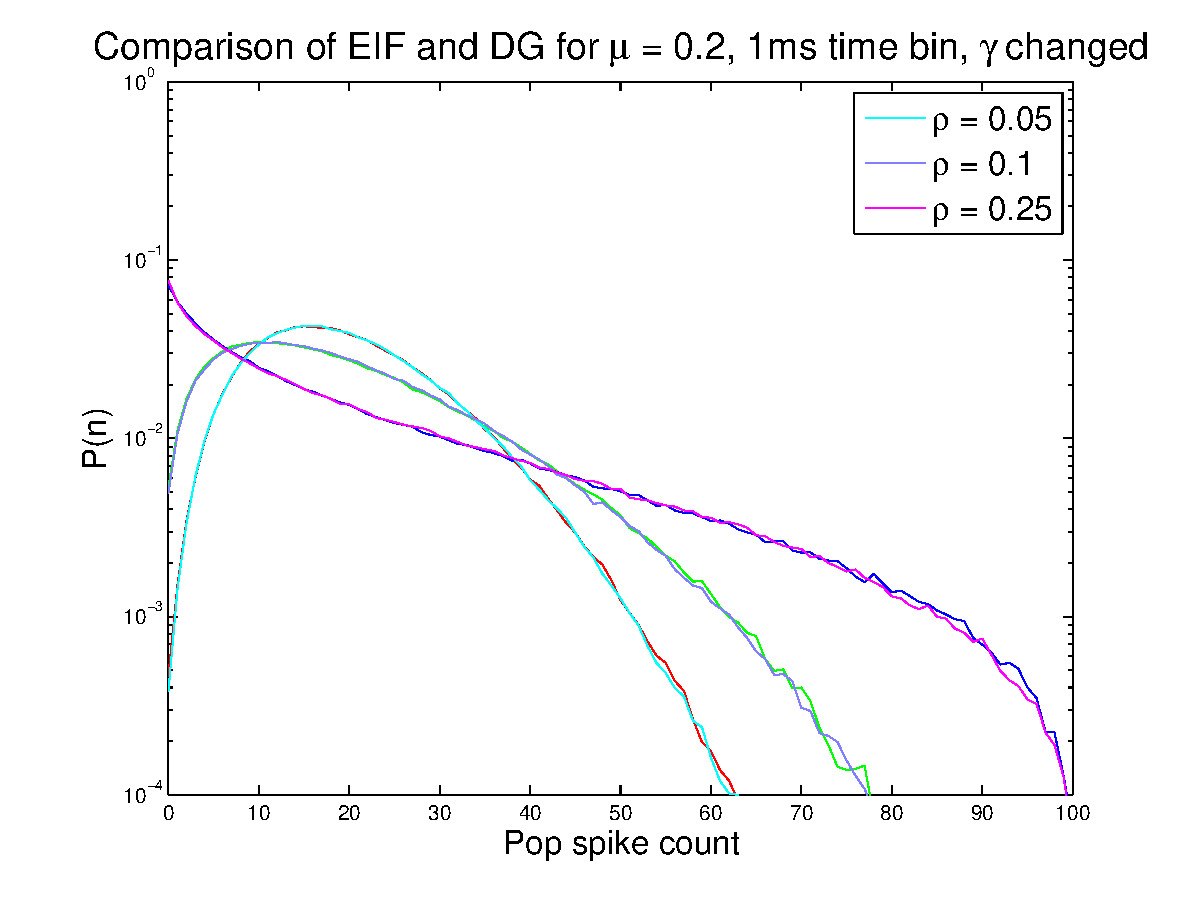
\includegraphics[width=0.75\textwidth]{../Figures/EIF/DG_EIF_Macke_2a_mu_02_1ms_semilog}
\caption{\footnotesize We plot the DG probability distribution over the EIF probability distribution. We use a $1$ms time bin. Noise variance $\sigma = 6.23$. To achieve  a mean firing rate $\mu = 0.2$ we raise $\gamma =-12$mV. The values of $\lambda = 0.33,~0.54,~0.842$. Values for the DG are: $\sigma = 1$, $\gamma = -0.84$, $\lambda = 0.1,~0.19,~\text{and}~0.435$.}\label{figdgeif}
\end{figure}

%%%%%%%%%%%%%
% Changing ref period   %
%%%%%%%%%%%%%
\begin{figure}[H]
\centering
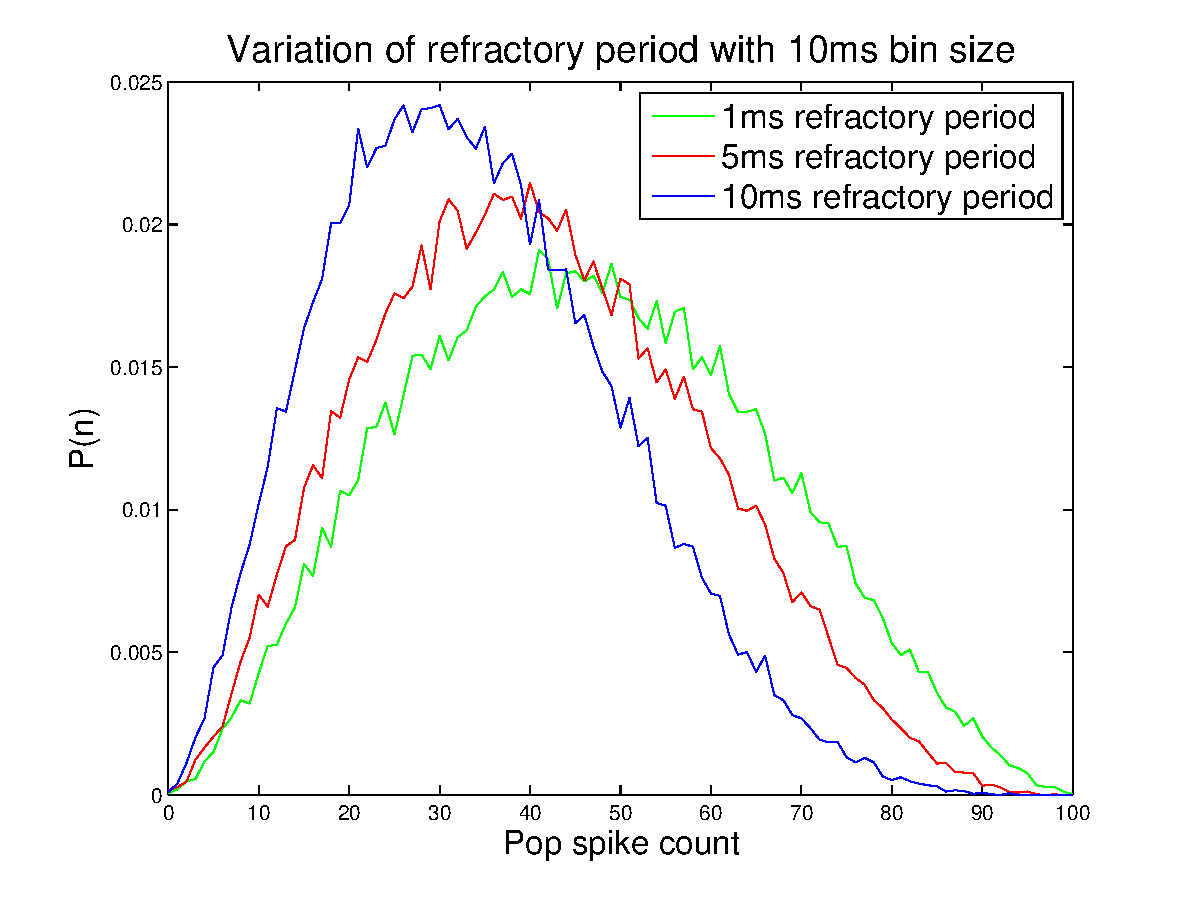
\includegraphics[width=0.75\textwidth]{../Figures/EIF/Refractory_period_10ms_bin}
\caption{\footnotesize Mean firing rates increases with decreasing refractory period. Mean firing rates: $\mu = 0.46,~0.40,~0.34$ and correlations $\rho = 0.14,~0.12,~0.10$ for refractory periods $\tau_\text{ref} = 1$ms, $5$ms, $10$ms. Everything except the refractory periods was held constant.}
\label{figdgeif}
\end{figure}

\subsection{Using values to try ``break'' DG}
Not possible. Varying the parameters serves to constrain the possible values of $\mu$ and $\rho$. It does not alter the shape of the probability distribution for a fixed $\mu$ and $\rho$.

%%%%%%%%%%%
\section{Linear filter}%
%%%%%%%%%%%
\begin{enumerate}
\item Describe numerical algorithm/simulations.
\item Two methods of generating spikes: $r_\text{est} \Delta t$ and integrating the firing rate until a random variable is reached.
\item Describe method we use to match the means and correlations.
\item Curves showing how output correlations vary with input covariance.
\item Static non-linearity plot?
\item High firing rate leads to double counting
\item Low firing rate over-estimates zeros
\item Linear filter gives gaussian firing rate
\item Firing rate gives rise to spikes 
\end{enumerate}


We can imagine our $N$ neurons receiving common input as being $N$ different trials, where the common input is identical from trial to trial and the independent input is uncorrelated from trial to trial. We treat the common input as the ``signal'' and the independent input as background noise. We approximate the firing rate of the EIF neuron first by a linear filter applied to the input signal and then by a linear-nonlinear cascade. See~\cite{Ostojic:2011kf} for this description, and for the numerical methods~\cite{Richardson:2007ct}.

Using a linear-nonlinear cascade the firing rate is approximated as:
\begin{equation}
r(t) = F\left(A(t) * c(t) \right),
\end{equation}
where $F$ is the static non-linearity, $A(t)$ is the linear filter, and $c(t)$ is the common input: $c(t) = \sqrt{\sigma^2 \tau \lambda}~\xi(t)$ . In the linear limit the firing rate is given by:
\begin{equation}
r(t) = r_0 + A(t) * c(t).
\end{equation} 

The static non-linearity is:
\begin{equation}
F(L) = \Phi\left( \gamma + \frac{L}{A_0}\right),\quad \text{where}\quad A_0 = \int_0^\infty \dd \tau A(\tau),
\end{equation}
and $\Phi$ is the transfer function of the neuron.

The estimated firing rate has mean and variance:
\begin{align}
\mathbb{E}\left[ r(t) \right]~~\!&= r_0 ,\\
\mathbb{E}\left[ r^2(t) \right]&= \sigma^2\tau\lambda \int_0^\infty A^2(\tau) \dd \tau = \sigma_r^2,
\end{align}
and so can be described by a a Gaussian $\mathcal{N}(r_0,\sigma_r^2)$.

\subsection{Spike probabilities}
For homogeneous neurons:
\begin{align}
P_\text{DG}(k) = \nchoosek
\end{align}

\begin{figure}[H]
	\centering
	\begin{subfigure}[h]{0.49\textwidth}
	\centering
	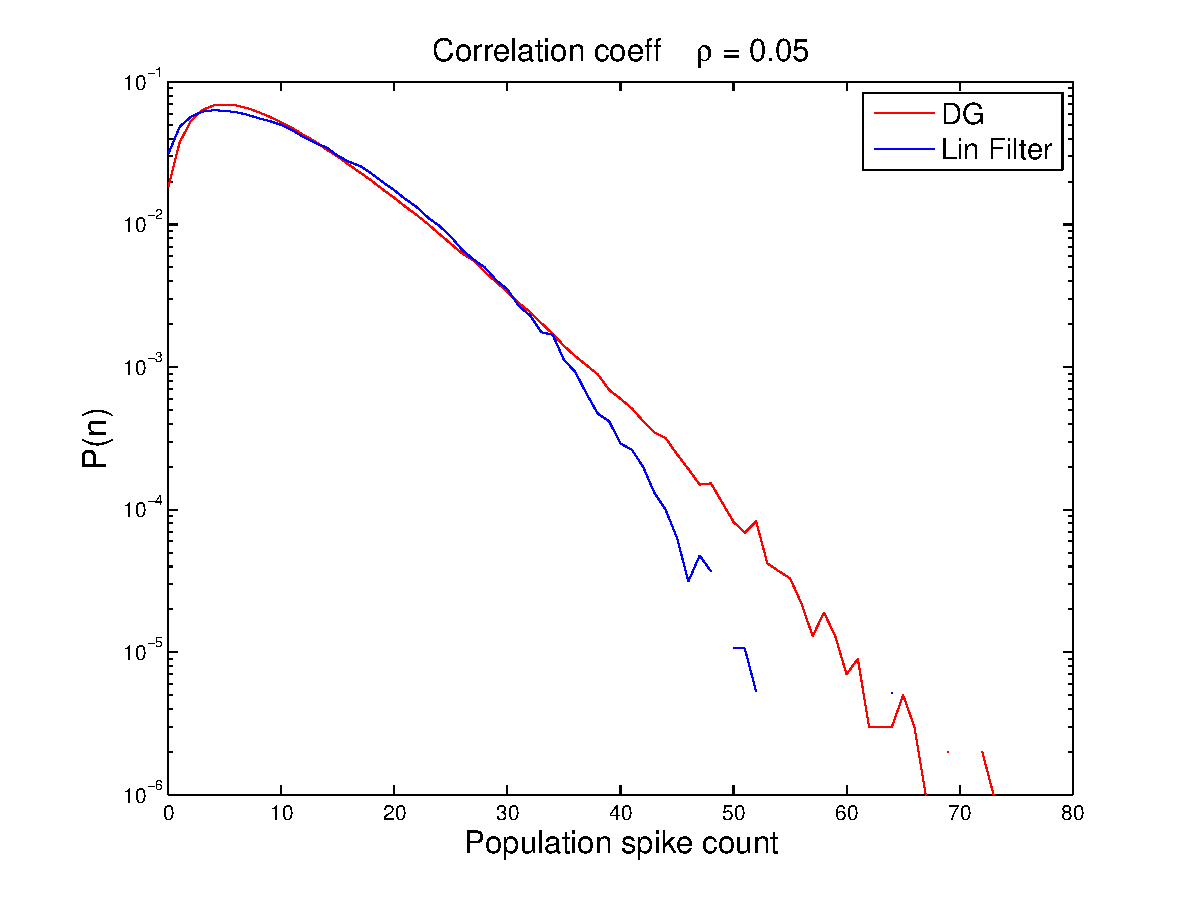
\includegraphics[width=\textwidth]{../Figures/Lin_Filter/Filt_DG_indiv_mu_01_rho_05}
	\label{fig11}
	\end{subfigure}
	\begin{subfigure}[h]{0.49\textwidth}
	\centering
	\includegraphics[width=\textwidth]{../Figures/Lin_Filter/Filt_DG_indiv_mu_01_rho_1}
	\label{fig11}
	\end{subfigure}\\
	\begin{subfigure}[h]{0.66\textwidth}
	\centering
	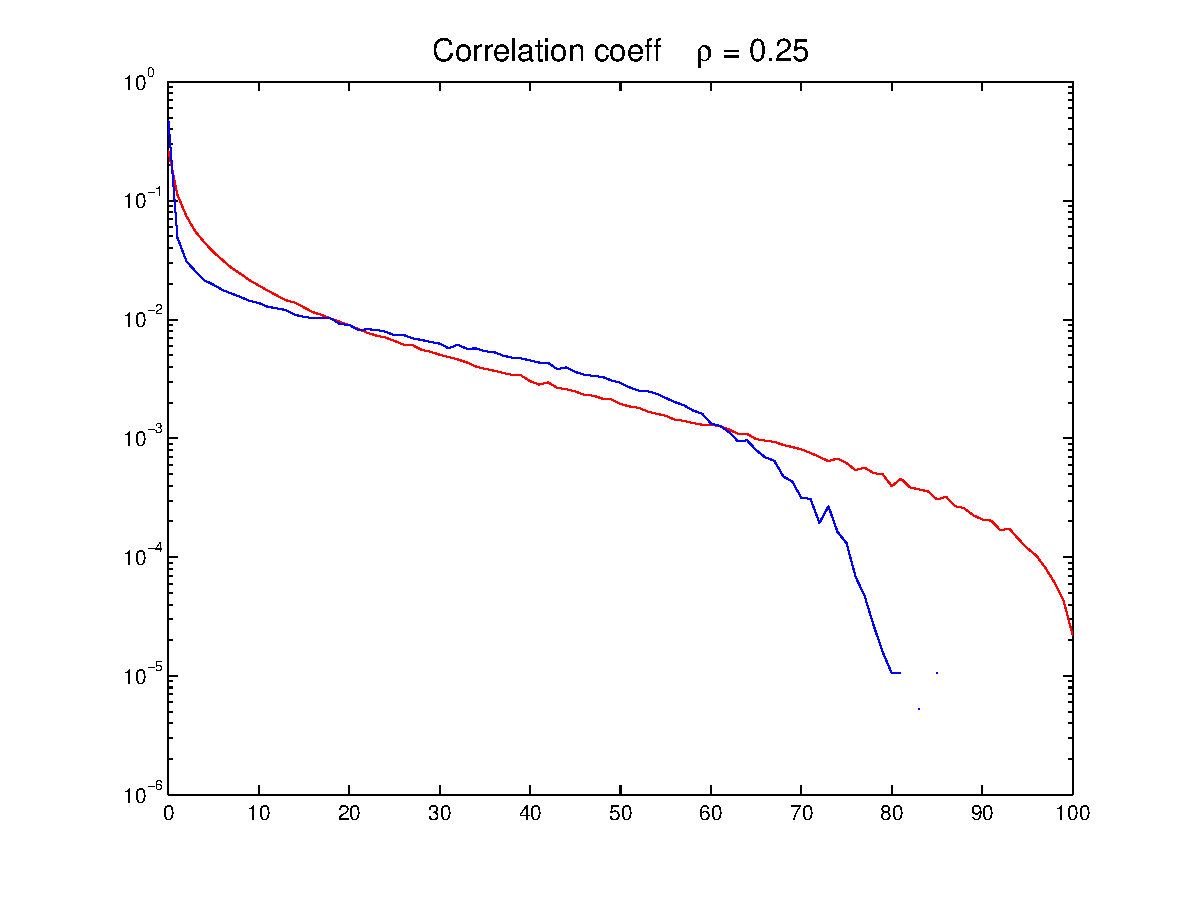
\includegraphics[width=\textwidth]{../Figures/Lin_Filter/Filt_DG_indiv_mu_01_rho_25}
	\label{fig12}
	\end{subfigure}
	\caption{\footnotesize Linear-nonlinear cascade. Mean firing rate of $\mu = 0.1$.}
\end{figure}

\begin{figure}[H]
	\centering
	\begin{subfigure}[h]{0.49\textwidth}
	\centering
	\includegraphics[width=\textwidth]{../Figures/Lin_Filter/Filt_DG_indiv_mu_01_rho_05_gamma_changed}
	\label{fig11}
	\end{subfigure}
	\begin{subfigure}[h]{0.49\textwidth}
	\centering
	\includegraphics[width=\textwidth]{../Figures/Lin_Filter/Filt_DG_indiv_mu_01_rho_1_gamma_changed}
	\label{fig11}
	\end{subfigure}\\
	\begin{subfigure}[h]{0.66\textwidth}
	\centering
	\includegraphics[width=\textwidth]{../Figures/Lin_Filter/Filt_DG_indiv_mu_01_rho_25_gamma_changed}
	\label{fig12}
	\end{subfigure}
	\caption{\footnotesize In this case we have fixed the noise strength at $\sigma = 6.23$ and varied $\gamma$ in order to achieve the usual mean firing rate etc. Linear-nonlinear cascade. Mean firing rate of $\mu = 0.1$.}
\end{figure}

\begin{figure}[H]
	\centering
	\begin{subfigure}[h]{0.49\textwidth}
	\centering
	\includegraphics[width=\textwidth]{../Figures/Lin_Filter/Filt_DG_indiv_lin_mu_01_rho_05}
	\label{fig11}
	\end{subfigure}
	\begin{subfigure}[h]{0.49\textwidth}
	\centering
	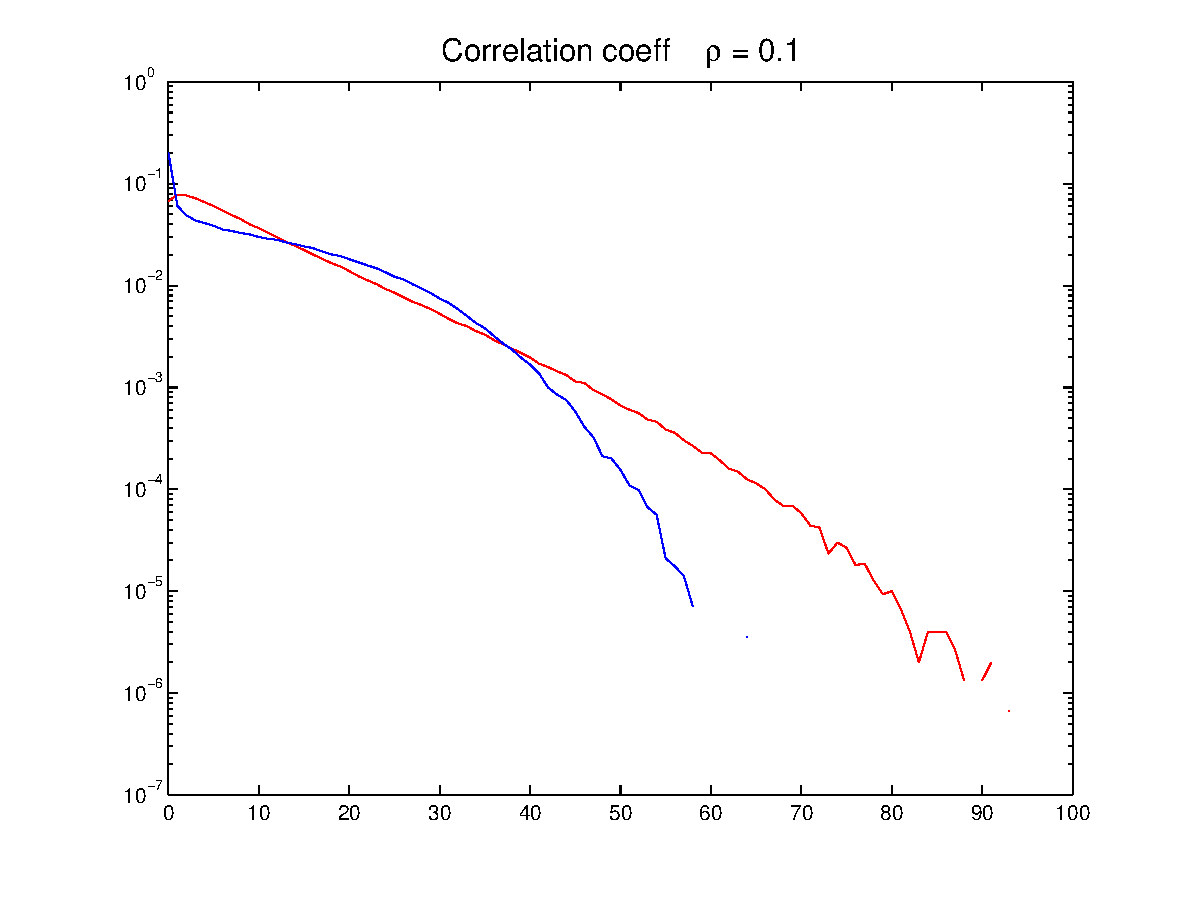
\includegraphics[width=\textwidth]{../Figures/Lin_Filter/Filt_DG_indiv_lin_mu_01_rho_1}
	\label{fig11}
	\end{subfigure}
	\caption{\footnotesize Linear filter, with values... . It is not possible to achieve a correlation of $\rho = 0.25$.}
\end{figure}

\begin{enumerate}
\item Nonlinearity goes to step function for very low firing rates.
\item The tail drops off too quickly -- reason why this is: we have multiple spikes per bin and we truncate these to return to just one spike per bin. This will have little effect on small population spike counts, but large population spike counts are penalized quite a bit.
\item If the probability of a spike in a bin is $p$ then the probability of two spikes in a bin is $p^2$ and the ratio $p^2/p = p$. So it is unavoidable having approximately $10\%$ of bins with multiple spikes.
\item Can we try without worrying about double counting? Let it be?
\item Nonlinearity helps with double counting.
\item Doomed without refractory period.
\item Feedback kernel method for refractory period could solve this problem but we don't do this.
\end{enumerate}

\begin{enumerate}
\item Use the $D_{\text{KL}}$ to quantify the match.
\end{enumerate}


%%%%%%%%%%%%%%%%
\bibliography{../papers_bib}{}  %
\bibliographystyle{plain}           %
%%%%%%%%%%%%%%%%
\end{document}